\documentclass[11pt, oneside]{article} 
\usepackage{geometry}
\geometry{letterpaper} 
\usepackage{graphicx}
	
\usepackage{amssymb}
\usepackage{amsmath}
\usepackage{parskip}
\usepackage{color}
\usepackage{hyperref}

\graphicspath{{/Users/telliott/Github/figures/}}
% \begin{center} \includegraphics [scale=0.4] {gauss3.png} \end{center}

\title{Limits and continuity}
\date{}

\begin{document}
\maketitle
\Large

%[my-super-duper-separator]

\subsection*{Limit concept}
Consider the graph of a function $f(x)$.  We might choose a power of $x$ similar to $y = x^2$ or $y = x^3 - x$, which affirmatively has two properties that are of interest here:  continuity and differentiability (we'll get to those ideas in a bit).  Let's just say $y=f(x)$ is a "good" function.  The functions we deal with in this book are all "good."

\begin{center} 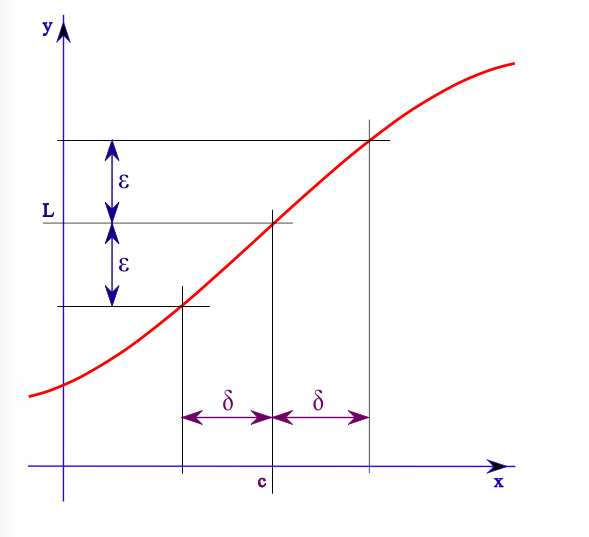
\includegraphics [scale=0.35] {epsilon-delta.png} \end{center}
Focus on the neighborhood of a point on the $x$-axis, $x=c$.

By inspection of the graph, for points near $c$, the value of $f$ at those points is not too different from $L$.

(It is also true here that the value of $f(x)$ at $c$ is equal to $L$.  This matters for continuity but not for limits).

We would like to say that the \emph{limit} of $f(x)$ as $x$ \emph{approaches} $c$ is equal to $L$.  The idea is that we can make $f(x)$ as close to $L$ as we please, provided we choose $x$ sufficiently close to $c$.

\begin{quote}When the values successively attributed to a variable approach indefinitely to a fixed value, in a manner so as to end by differing from it by as little as one wishes, this last is called the limit of all the others.  ---Cauchy\end{quote}

\begin{center} 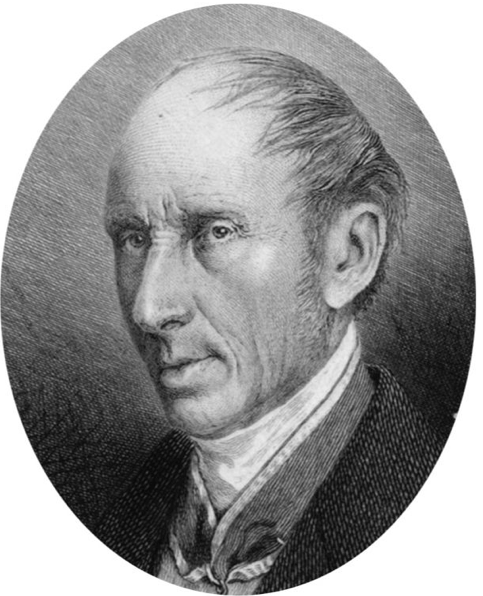
\includegraphics [scale=0.3] {Cauchy} \end{center}

Modern mathematicians don't like that word "approach", which conjures up movement and the involvement of time.

They also don't like reasoning from what they see in a graph, in part because no graph can show the whole function for the general case.  To free ourselves from graphs and pictures, we will use an algebraic method from the formal apparatus of calculus.

There are two equivalent approaches, neighborhoods, and epsilon-delta formalism.  Let's look at neighborhoods briefly.

\subsection*{neighborhoods}

First, an \emph{interval} between two real numbers $a$ and $b$ ($a < b$) contains every real number $a < x < b$.
\[ (a,b) = x \ | \ a < x < b \]

The "$|$" means $x$ "such that" the condition $a < x < b$ holds.

A \emph{closed} interval $[a,b]$ includes the endpoints, $a \le x \le b$, while an \emph{open} interval $(a,b)$ excludes them.  Half-open intervals like $[a,b)$ may be defined, and an interval with $\pm \ \infty$ as an endpoint is always open on that end, for example:  $[a,\infty)$, because infinity \emph{is not a number}.

Any open interval with a point $p$ as its midpoint is called a \emph{neighborhood} of $p$.  Let $r$ be the distance from $p$ to the boundary of a particular neighborhood;  $r$ may be large or very very small.  We denote a neighborhood of $p$ as $N(p)$.  $N(p)$ consists of all those values of $x$ such that

\[  |x-p| < r \].

which we would write more formally as

\[ N(p) = x \ | \ |x-p| < r \].

To say that the limit $f(x) \rightarrow L$ exists, we mean that for every neighborhood $N_1(L)$, no matter how small, there exists some neighborhood $N_2(p)$ such that $f(x)$ is contained within $N_1(L)$, written as

\[ f(x) \in N_1(L) \]

whenever $x \in N_2(p)$.  

If $N_1(L)$ is very small, then $N_2(p)$ may need to be very small as well, to guarantee that $f(x)$ is contained within $N_1$.  Here is an example where this condition is satisfied.

\begin{center} 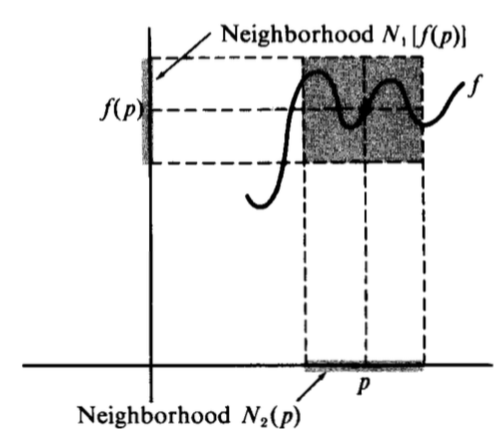
\includegraphics [scale=0.4] {neighborhood.png} \end{center}

The idea of a neighborhood is a nice abstraction to hide the apparatus of modern calculus, which we save for the Addendum.

An important fact about limits has to with the case where $x=p$.  It is \emph{not} necessary that $f(p) = L$.  This relaxed condition is in fact crucial for calculus.

\subsection*{example 1}

Limits can be easy or hard, depending on the problem.  Here is one found in the previous chapter on difference quotients:

\[ \lim_{h \rightarrow 0} \frac{2xh + h^2}{h} \]

When you see something like this, what you are supposed to do is reason about what happens as the variable $h$ approaches $0$ (gets smaller and smaller).  The first step in that is to figure out what would happen if $h$ actually would become zero.

Here, each term has a limit of $0$ when $h$ is zero, so we will have $0/0$.  The zero on the bottom is trouble, it means that the expression becomes undefined.

However, suppose we first cancel $h$ on top and bottom to obtain
\[ \lim_{h \rightarrow 0} \frac{2x + h}{1} = \lim_{h \rightarrow 0} \ 2x + h \]

Now, the answer is just $2x$.  This is valid as long as $h$ approaches zero but is never actually equal to it.  

Recall that we can have a limit for $f(x)$ as $x$ approaches $c$, even if $f(c)$ does not exist.

\subsection*{example 2}

Here is another important expression.  What is the value of $f(x)$ as $h$ approaches zero?

\[ \cos h < f(x) < \frac{1}{\cos h}  \]

Since $\cos 0 = 1$, the two outside terms both approach $1$ in the limit as $h$ approaches zero.  Since $f(x)$ lies between them, it must also approach $1$.

This is called the \emph{squeeze theorem}.

The magical thing is that this is true even if, when $h = 0$, $x = 0/0$.  We'll see this when we look at calculus of sine and cosine.

\subsection*{Continuity}

Continuity has an intuitive definition:  as Euler said, if we can graph a function \emph{without lifting our pencil from the paper}, then the function is continuous.

Here are some graphs showing examples of how continuity can fail.
\begin{center} 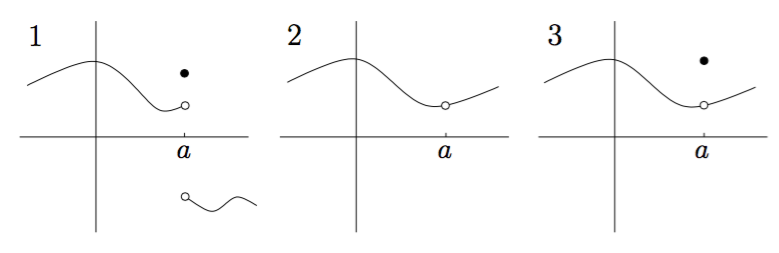
\includegraphics [scale=0.5] {continuity_failure.png} \end{center}
A filled circle means that the function yields that $y$-value for the corresponding $x$-value of the point, while an open circle means it does not.  The function may yield some other value, or simply be undefined. 
\begin{center} 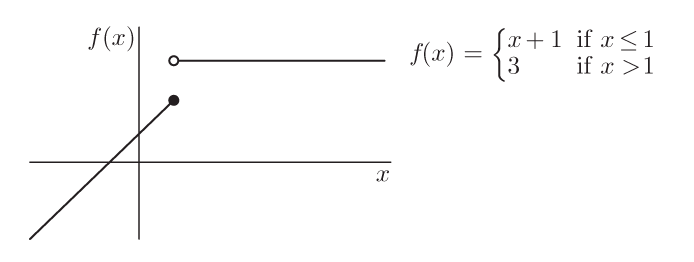
\includegraphics [scale=0.5] {continuity_failure2.png} \end{center}

For a function to be continuous at a point $x=c$, we imagine that if we vary $x$ in neighborhood of $c$, then $f(x)$ should not change in value by too much.

Again, we will call that value $L$, the limit of $f(x)$ as $x \rightarrow c$.  For $L$ to exist we require that the two one-sided limits be equal.  If we approach $c$ from the high side ($x > c$) or the low side ($x < c$), the limit must be the same.

Very important:  continuity requires, in addition, that $f(c)$ be equal to $L$.

\subsection*{Differentiability}

For a function to be differentiable, we require that the limit
\[ \lim_{h \rightarrow 0} \ \frac{f(x+h) - f(x)}{h} \]

exists.  An example of a function that is continuous but not differentiable at a particular point is the absolute value function.

\subsection*{example:  absolute value}
An algebraic definition of the absolute value function is piecewise:
\[ |x| =
\begin{cases}
\ \ x, \ \ \ x \ge 0  \\
-x, \ \ \ x < 0
\end{cases}
\]
\begin{center} 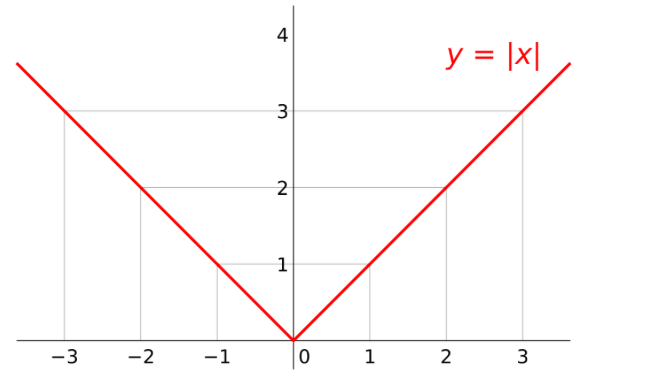
\includegraphics [scale=0.4] {abs.png} \end{center}

The function $f(x) = |x|$ is continuous at $x=0$ because the two one-sided limits exist and are equal to each other.  They are also equal to $f(0) = 0$.

However, there is no defined slope at $x=0$.  The difference quotient gives different results for positive $\Delta x$ (positive slope) than for negative $\Delta x$ (negative slope).

Without getting too technical

\begin{quote}Note that the graph of the absolute value function is "all in one piece", but has a "sharp point" at the origin. We will not attempt to make these descriptions precise, other than to say that the fact that the graph comes "all in one piece" is a feature of continuity, and that graphs of differentiable functions are "smooth" in that they do not have "sharp points." The unambiguous and demonstrably true statement here is that the absolute value function is continuous at 0 but is not differentiable at 0.\end{quote}

\url{https://oregonstate.edu/instruct/mth251/cq/Stage5/Lesson/diffVsCont.html}

\subsection*{practical limits}

$\bullet$ \ Plug in the value and see what happens.  No problem here:

\[ \lim_{x \rightarrow 2} \ \frac{x + 1}{x^2 + 3} = \frac{3}{7} \]

$\bullet$ \ Division by zero isn't allowed.  But we can factor:

\[ \lim_{x \rightarrow 3} \ \frac{x^2 - 9}{x - 3} = \lim_{x \rightarrow 3} \ \frac{(x + 3)(x - 3)}{x - 3} = \lim_{x \rightarrow 3} x + 3 = 6 \]

$\bullet$ \ Limit at infinity.  Convert to a limit at zero:

\[ \lim_{x \rightarrow \infty} \ \frac{x^2 + 3}{3x^2 + x + 1}= \lim_{1/x \rightarrow 0} \ \frac{1 + 3/x^2}{3 + 1/x + 1/x^2}  = \frac{1}{3} \]



\end{document}